\documentclass[12pt]{report}
\usepackage{graphicx}
\usepackage{listings}

% Document setup
\graphicspath{ {img/} }
\title{CSCI-476 Final Test}
\date{May 6, 2015}
\author{Gunnar Holwerda}
\renewcommand*\contentsname{Table of Contents}
\newcommand{\mychapter}[2]{
    \setcounter{chapter}{#1}
    \setcounter{section}{0}
    \chapter*{#2}
    \addcontentsline{toc}{chapter}{#2}
}

% Begin actual report

\begin{document}
\maketitle

\tableofcontents
\clearpage

\mychapter{1}{Executive Summary}
\section{Executive Summary}

\clearpage

% Begin Round 1

\mychapter{2}{Round 1}
\section{DiscoveredIn1655}
When starting out I was given the information that the members of mhk had been discussing RFC2100. This RFC mentions a few names, so I began using the names mentioned as subdomains of mthack.me and quickly found titan.mthack.me. I ran nmap on the host to see what ports were open.\\
	\begin{verbatim}
	$	nmap -sS -p1-65535 titan.mthack.me -v -T4
	\end{verbatim}
The nmap returned that port 22 and 23 were open. I attempted to ssh, but found that a public key was needed. Next I used telnet to connect to port 23 and was presented with my first flag ``DiscoveredIn1655''.\\
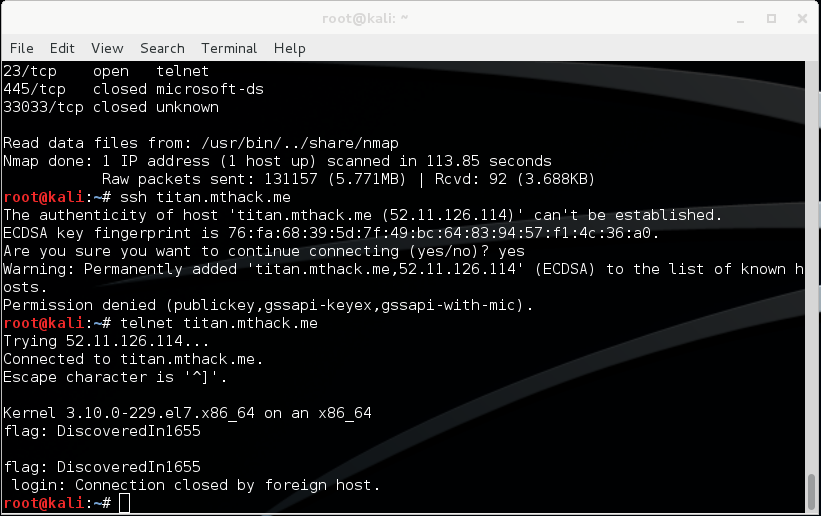
\includegraphics[scale=0.33, width=\linewidth]{DiscoveredIn1655.png}
\newline
\section{Th1sT1m3ItsAMoon}
In addition to titan.mthack.me, I was able to find the europa.mthack.me subdomain. After an nmap on europa I saw that port 7870 was open. There was no information about this port, so I used NetCat to connect to it, it returned ``SSH-2.0-OpenSSH\_6.6.1''. After seeing this I knew that I should use SSH to connect to europa.mthack.me on this port.
	\begin{verbatim}
	$	ssh europa.mthack.me -p 7870
	\end{verbatim}
After adding europa to my known\_hosts I was presented with my second flag ``Th1sT1m3ItsAMoon''.\\
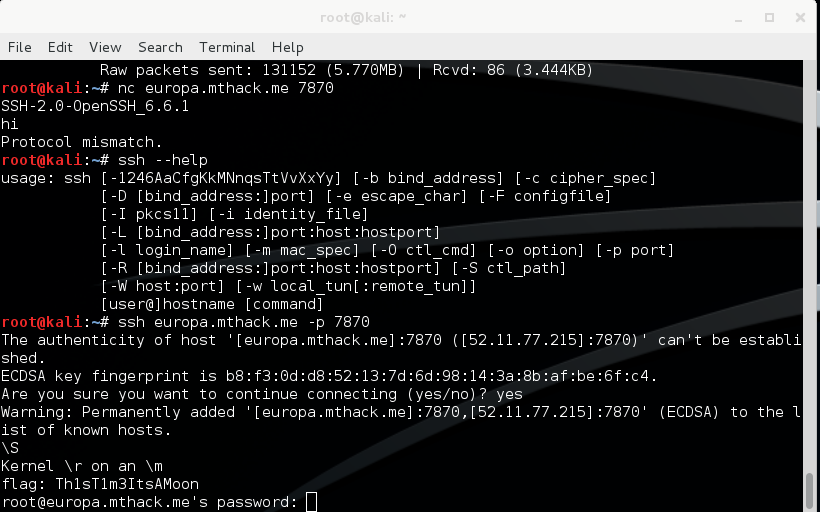
\includegraphics[scale=0.33, width=\linewidth]{Th1sT1m3ItsAMoon.png}
\newline
\section{SocialContract}
%
%	Text for SocialContractFlag
%
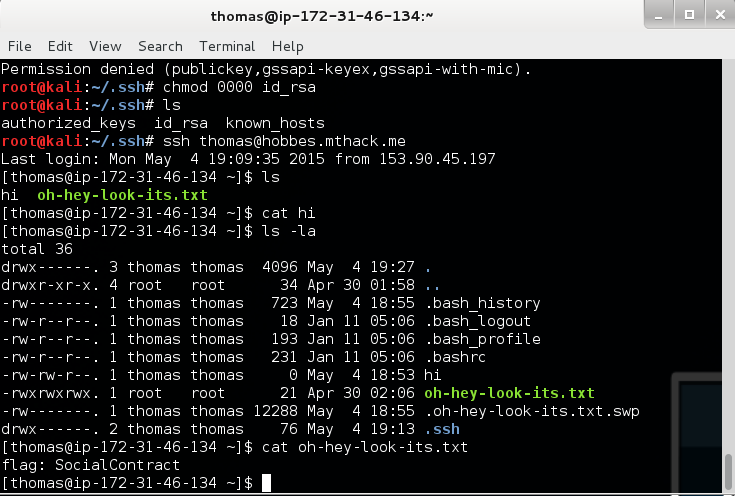
\includegraphics[scale=0.33, width=\linewidth]{SocialContract.png}

% Begin Round 2

\mychapter{3}{Round 2}
\section{TomcatIsAVulnerability}
%
%	Text for TomcatIsAVulnerability
%
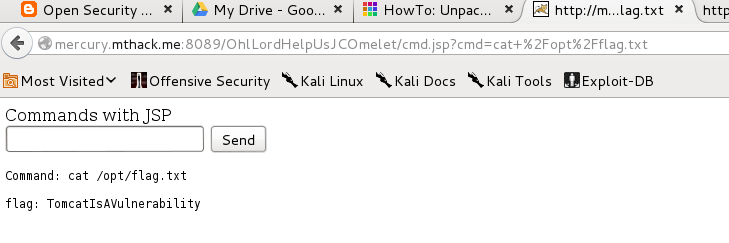
\includegraphics[scale=0.33, width=\linewidth]{TomcatIsAVulnerability.png}
\newline

% Begin Round 3

\mychapter{4}{Round 3}
\section{nextlevel}
Given the binary for round three, I first ran strings on the file using grep to try to find ``password'' or something along those lines. These attempts were unsuccessful, so I moved onto editing the binary using radare2. I was able to find the location of a ``jnz'' instruction right after asking for the number. I edited that instruction to be a ``jz'' instead and was presented with ``ciph3rfun.html''.\\

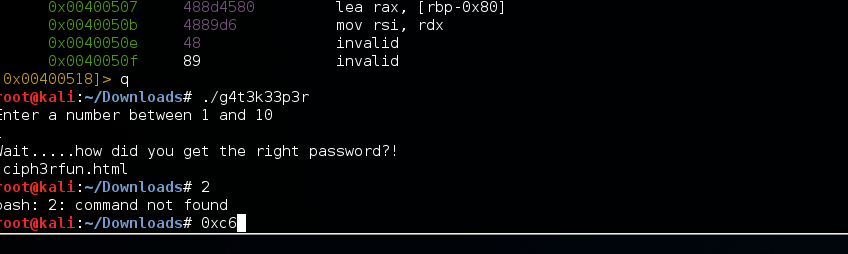
\includegraphics[scale=0.33, width=\linewidth]{ciph3rfunhtml.PNG}

I then visited www.mthack.me/ciph3rfun.html and was presented with some sort of enocded flag. It looked like ROT, so I went to a ROT decoder, entered the cipher text and was presented with the flag ``nextlevel''.\\
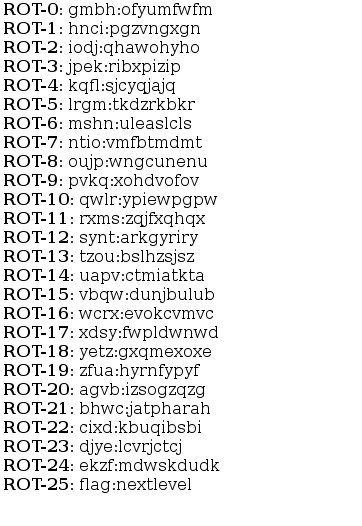
\includegraphics[scale=0.33, width=\linewidth]{nextlevel.PNG}
\newline

% Begin Round 4

\mychapter{5}{Round 4}
\section{FSInc3ption}
%
%	Text for FSInc3ption
%
	\begin{verbatim}
	# hydra ssh://192.168.2.12 -l user -P /usr/share/wordlists/metasploit/namelist.txt -v -t 8
	\end{verbatim}
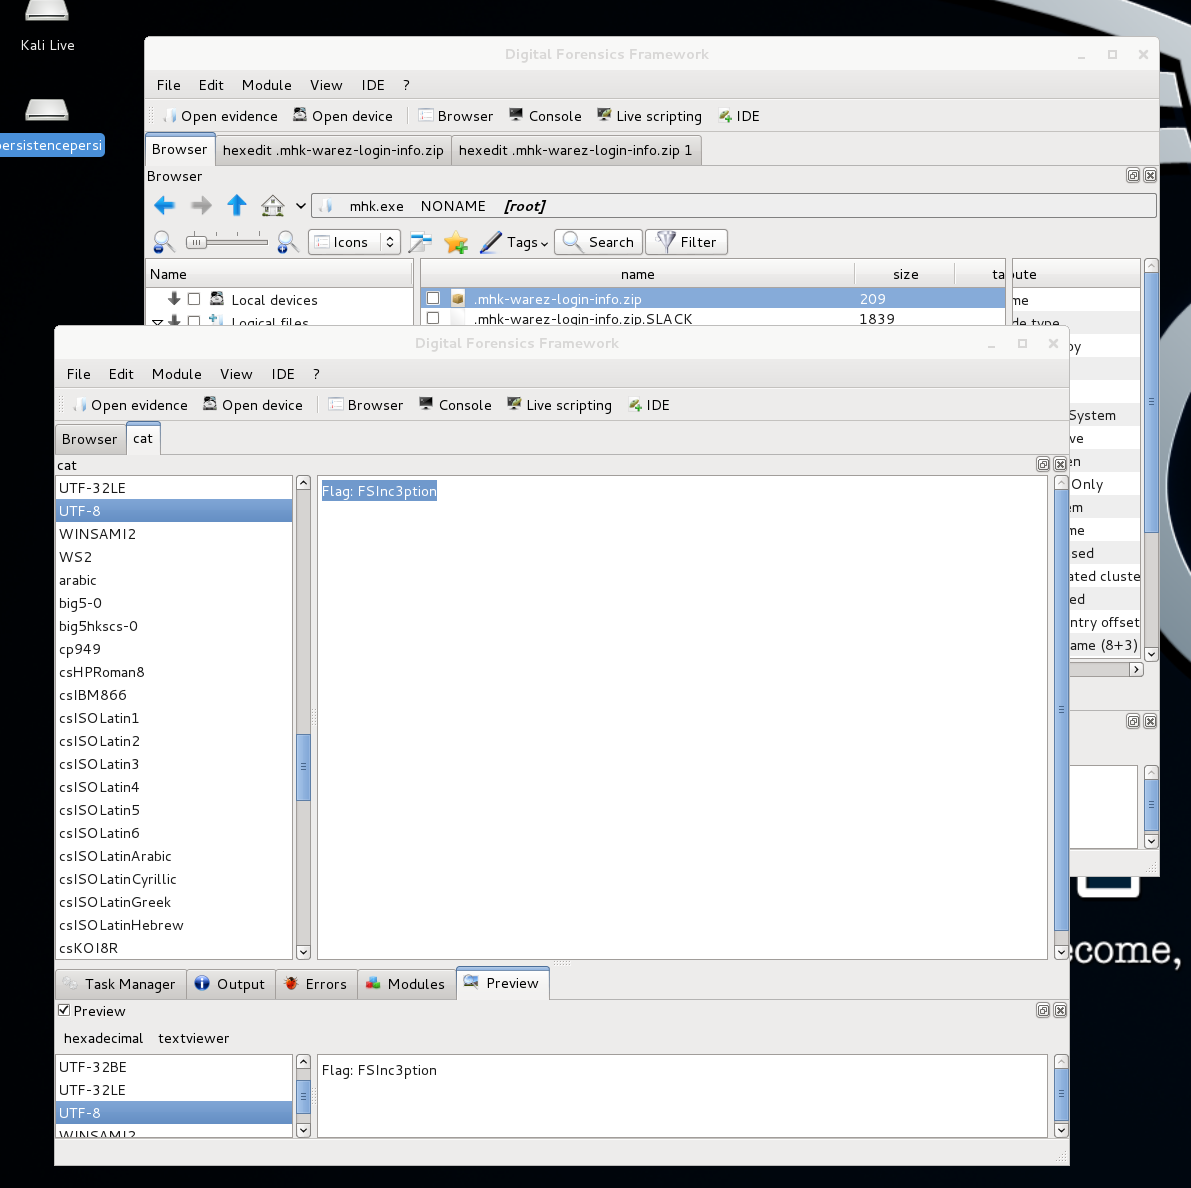
\includegraphics[scale=0.33, width=\linewidth]{FSInc3ption.PNG}
\newline
\section{deaddrop}
%
%	Text for deaddrop
%
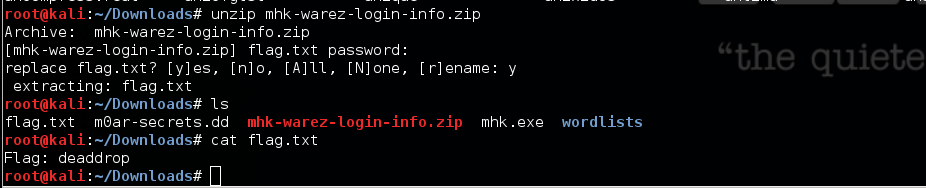
\includegraphics[scale=0.33, width=\linewidth]{deaddrop.png}
\newline

\mychapter{6}{Round 5}

\mychapter{7}{Misc. Flags}
\section{mylittlepwnie}
%
%	Text for mylittlepwnie
%
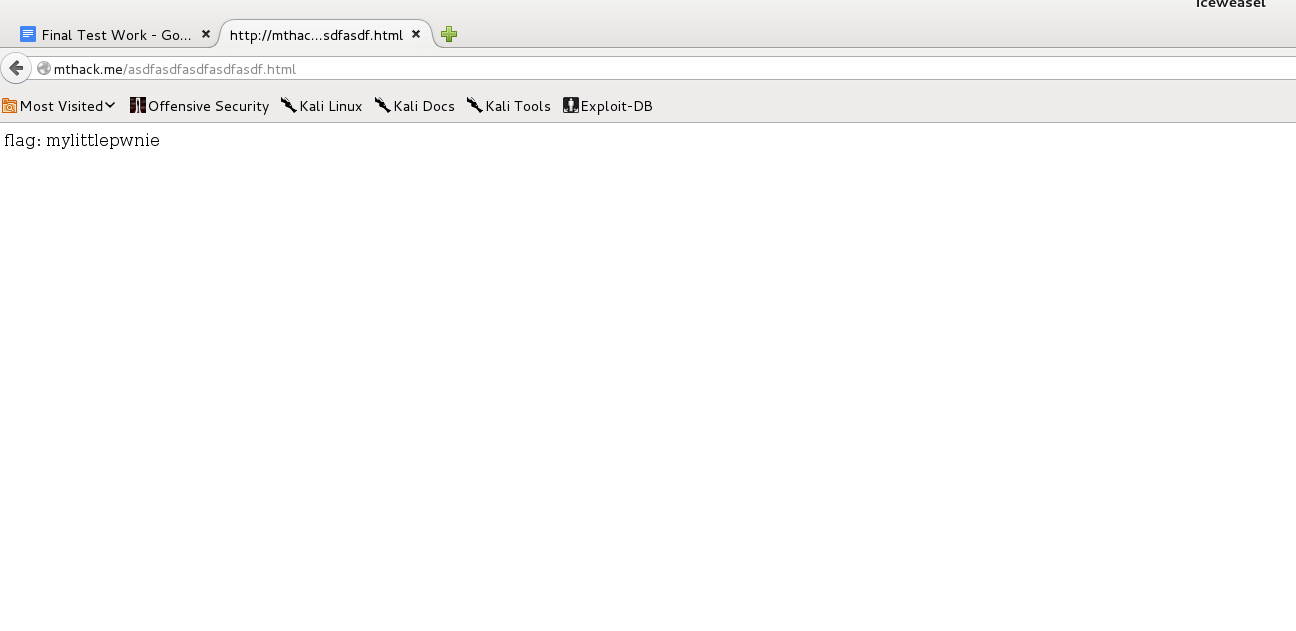
\includegraphics[scale=0.33, width=\linewidth]{mylittlepwnie.png}
\clearpage

\mychapter{8}{Summary}

\clearpage

\mychapter{9}{Bibliography}

\end{document}